\section{Analyse von Funktion F230: Bib\TeX -Export}
Diese Funktion gehört zur Komponente \textbf{View:Export}. Die für diesen Export nötigen Informationen sind vollständig in der Datenbank enthalten und müssen mit \gls{glos:django} ermittelt werden. Die so erhaltenen Daten werden dem Benutzer in einer View im \BibTeX -Format zum Kopieren angezeigt. Verdeutlicht wird dies in dem Sequenzdiagramm \ref{fig:BibTeX-Export}.

\begin{figure}[H]
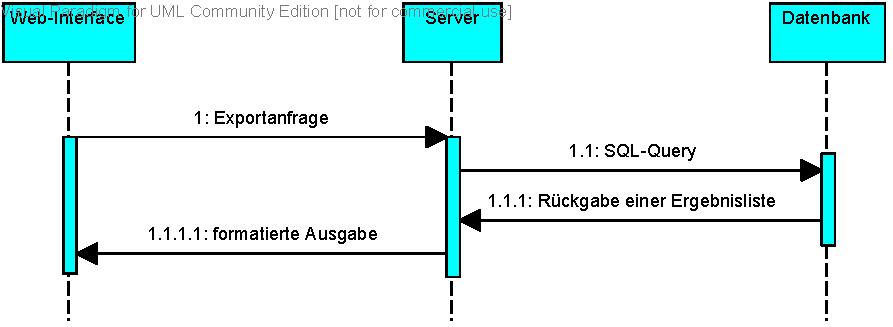
\includegraphics[width=0.8\linewidth]{bilder/Seq-BibTex.pdf}
\caption[BibTeX-Export]{BibTeX-Export}
\label{fig:BibTeX-Export}
\end{figure}

\section{Analyse von Funktion F231: Universitätsbibliothek-Export}

Diese Funktion muss in einer extra Klasse dargestellt werden. Die für diesen
Export nötigen Informationen sind vollständig in der Datenbank enthalten und
müssen mittels \gls{glos:django} ermittelt werden. Diese Daten
werden durch eine Funktion in das richtige Format gebracht und in einem vom
Benutzer vorher gewählten Dateipfad in einem Allegro kompatiblen Format
gespeichert. Diese Komponente gehört ebenfalls zur Komponente
\textbf{View:Export}. Veranschaulicht wird der Vorgang in dem Sequenzdiagramm
\ref{fig:Allegro-Export}.

\begin{figure}[H]
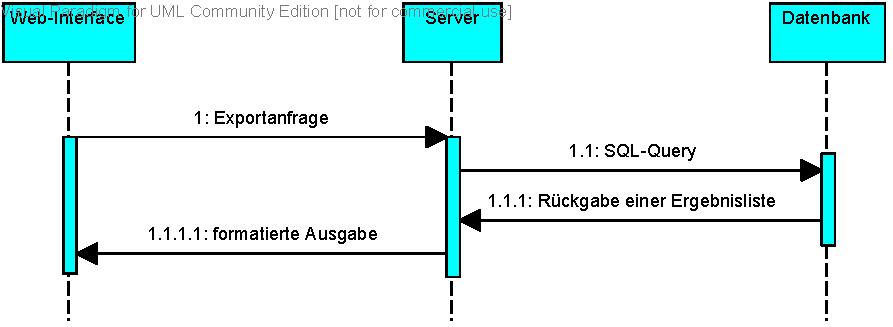
\includegraphics[width=0.8\linewidth]{bilder/Seq-BibTex.pdf}
\caption[Allegro-Export]{Allegro-Export}
\label{fig:Allegro-Export}
\end{figure}

\section{Analyse von Funktion F300: Benutzerverwaltung}
Alle Informationen zu den Benutzern werden in einer Datenbank gespeichert. Änderungen an bestehenden Benutzern und das Hinzufügen neuer Benutzer wird durch ein Webformular von einem Benutzer mit ausreichenden Rechte eingeleitet. Mithilfe von \gls{glos:django} werden die Informationen aus dem Formular gelesen und alle Änderungen in der Datenbank eingetragen. Das Sequenzdiagramm ist trivial, da nur einfach Frage/Antwort-Vorgänge zwischen Server und Datenbank stattfinden. Diese Komponente gehört zur Komponente \textbf{Admin}.

\begin{figure}[H]
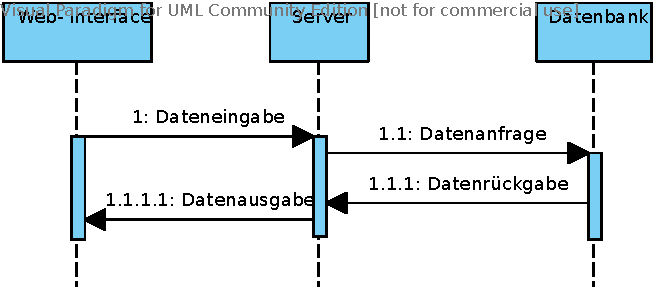
\includegraphics[width=0.8\linewidth]{bilder/f300.pdf}
\caption[Benutzerverwaltung]{Benutzerverwaltung}
\label{fig:300}
\end{figure}

In dem Diagramm sieht man, dass zuerst die Rechte als Dateneingabe in das
System gegeben werden, diese dann an den Server weitergegeben werden. Der
Server richtet dann die Änderungsanfrage an die Datenbank und bekommt entweder
eine Bestätigung oder eine entsprechende Fehlermeldung, die er an das
Web-Interface zurückgibt.

\section{Analyse von Funktion F301: Rechtezuweisung für Rollen}
Die Rechte einer Rolle werden in einer eigenen Tabelle der Datenbank gespeichert. Ein Benutzer mit ausreichenden Rechten kann über ein Webformular Änderungen eingeben. Diese Änderungen werden mithilfe von \gls{glos:django} aus dem Webformular ausgelesen und in der Tabelle der Datenbank gespeichert. Das Sequenzdiagramm ist trivial, da nur einfach Frage/Antwort-Vorgänge zwischen Server und Datenbank stattfinden. Diese Funktion gehört zur Komponente \textbf{Admin}.


\begin{figure}[H]
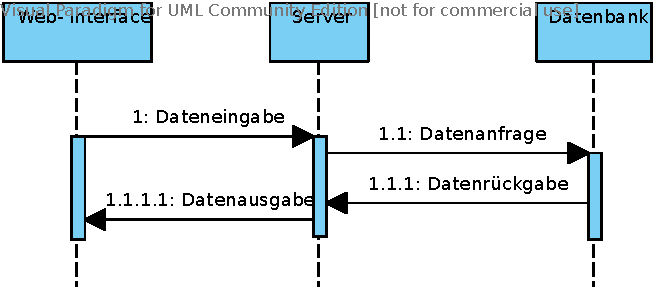
\includegraphics[width=0.8\linewidth]{bilder/f300.pdf}
\caption[Rechtezuweisung für Rollen]{Rechtezuweisung für Rollen}
\label{fig:301}
\end{figure}

In dem Diagramm sieht man, dass die Änderungen der Rollenrechte zuerst im
Web-Interface eingegeben werden und diese als Datenpaket an den Server
übermittelt. Dieser wertet die Daten aus und stellt eine entsprechende
Änderungsanfrage an die Datenbank. Er verarbeitet die aus einer Fehlermeldung
oder einer Bestätigung bestehende Antwort und gibt eine entsprechende
Ausgabemeldung an das Web-Interface zurück.

\section{Analyse von Funktion F302: Benutzer Rolle(n) zuweisen}
Die Rollen eines Benutzer werden in einer speziellen Tabelle in der Datenbank gespeichert. Ein Benutzer mit ausreichenden Rechten kann über ein Webformular Änderungen eingeben. Diese Änderungen werden mithilfe von \gls{glos:django} aus dem Formular ausgelesen und in der entsprechenden Datenbank gespeichert. Das Sequenzdiagramm ist trivial, da nur einfach Frage/Antwort-Vorgänge zwischen Server und Datenbank stattfinden. Diese Funktion gehört zur Komponente \textbf{Admin}.

\begin{figure}[H]
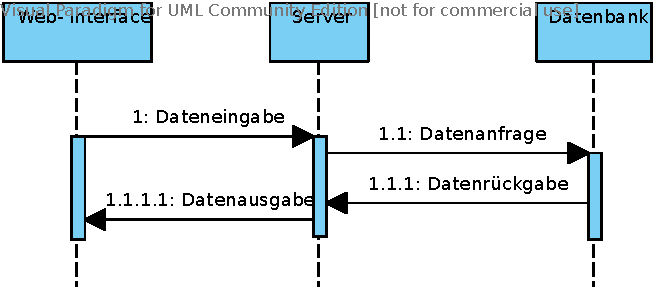
\includegraphics[width=0.8\linewidth]{bilder/f302.pdf}
\caption[Benutzer Rolle(n) zuweisen]{Benutzer Rolle(n) zuweisen}
\label{fig:302}
\end{figure}

In dem Sequenzdiagram sieht man, dass die Änderungen an der Relation zuerst im
Web-Interface eingegeben und dann an den Server übermittelt werden. Dieser
überprüft sie und schickt eine passende Änderungsanfrage an die Datenbank.
Diese verarbeitet die Anfrage und gibt dem Server entweder eine Bestätigung
oder eine Fehlermeldung zurück, die dieser in eine Ausgabe umwandelt und an das
Web-Interface weiterreicht.
